\def\mytitle{ASSIGNMENT}
\def\myauthor{Gajula Arun Kumar}
\def\contact{arunkumarg099@gmail.com}
\def\mymodule{Future Wireless Communications (FWC)}
\documentclass[journal,12pt,twocolumn]{IEEEtran}

\usepackage{setspace}
\usepackage{gensymb}
\usepackage{xcolor}
\usepackage{caption}
\usepackage[hyphens,spaces,obeyspaces]{url}
\usepackage[cmex10]{amsmath}
\usepackage{mathtools}
\singlespacing
\usepackage{amsthm}
\usepackage{mathrsfs}
\usepackage{txfonts}
\usepackage{stfloats}
\usepackage{cite}
\usepackage{cases}
\usepackage{subfig}
\usepackage{longtable}
\usepackage{multirow}
\twocolumn


\usepackage{graphicx}
\graphicspath{{./images/}}
\usepackage[colorlinks,linkcolor={black},citecolor={blue!80!black},urlcolor={blue!80!black}]{hyperref}
\usepackage[parfill]{parskip}
\usepackage{lmodern}
\usepackage{tikz}
\usepackage{circuitikz}
\usepackage{karnaugh-map}
\usepackage{pgf}
\usepackage[hyphenbreaks]{breakurl}

\usepackage{tabularx}
\usetikzlibrary{calc}

\renewcommand*\familydefault{\sfdefault}
\usepackage{watermark}
\usepackage{lipsum}
\usepackage{xcolor}
\usepackage{listings}
\usepackage{float}
\usepackage{titlesec}
\DeclareMathOperator*{\Res}{Res}
%\renewcommand{\baselinestretch}{2}
\renewcommand\thesection{\arabic{section}}
\renewcommand\thesubsection{\thesection.\arabic{subsection}}
\renewcommand\thesubsubsection{\thesubsection.\arabic{subsubsection}}

\renewcommand\thesectiondis{\arabic{section}}
\renewcommand\thesubsectiondis{\thesectiondis.\arabic{subsection}}
\renewcommand\thesubsubsectiondis{\thesubsectiondis.\arabic{subsubsection}}

% correct bad hyphenation here
\hyphenation{op-tical net-works semi-conduc-tor}

\titlespacing{\subsection}{1pt}{\parskip}{3pt}
\titlespacing{\subsubsection}{0pt}{\parskip}{-\parskip}
\titlespacing{\paragraph}{0pt}{\parskip}{\parskip}
\newcommand{\figuremacro}[5]{
    \begin{figure}[#1]
        \centering
        \includegraphics[width=#5\columnwidth]{#2}
        \caption[#3]{\textbf{#3}#4}
        \label{fig:#2}
    \end{figure}
}

\lstset{
frame=single, 
breaklines=true,
columns=fullflexible
}

%\thiswatermark{\centering \put(400,-128.0){\includegraphics[scale=0.3]{logo}} }
\title{\mytitle}
\author{\myauthor\hspace{1em}\\\contact\\IITH\hspace{0.5em}-\hspace{0.6em}\mymodule}
\date{20-12-2022}
\def\inputGnumericTable{}                                 %%
\lstset{
%language=C,
frame=single, 
breaklines=true,
columns=fullflexible
}
 

\begin{document}
%

\theoremstyle{definition}
\newtheorem{theorem}{Theorem}[section]
\newtheorem{problem}{Problem}
\newtheorem{proposition}{Proposition}[section]
\newtheorem{lemma}{Lemma}[section]
\newtheorem{corollary}[theorem]{Corollary}
\newtheorem{example}{Example}[section]
\newtheorem{definition}{Definition}[section]
%\newtheorem{algorithm}{Algorithm}[section]
%\newtheorem{cor}{Corollary}
\newcommand{\BEQA}{\begin{eqnarray}}
\newcommand{\EEQA}{\end{eqnarray}}
\newcommand{\define}{\stackrel{\triangle}{=}}
\bibliographystyle{IEEEtran}

\vspace{3cm}
  \maketitle
  \tableofcontents
 
\section{Question}  
      A logic circuit implements the boolean function F=X'.Y+X.Y'.Z'. It is found that the input combination X=Y=1 can never occur. Taking this into account, a simplified expression for F is given by



  \section{Components}
  \begin{tabularx}{0.4\textwidth} { 
  | >{\centering\arraybackslash}X 
  | >{\centering\arraybackslash}X 
  | >{\centering\arraybackslash}X
  | >{\centering\arraybackslash}X | }
\hline
 \textbf{Component}& \textbf{Values} & \textbf{Quantity}\\
\hline
Arduino & UNO & 1 \\  
\hline
JumperWires& M-M & 10 \\ 
\hline
Breadboard &  & 1 \\
\hline
LED & &2 \\
\hline
Resistor &220ohms & 1\\
\hline
\end{tabularx}



\begin{center}
Figure.a
\end{center}

\section{Truth Table}
  \begin{tabularx}{0.46\textwidth} { 
  | >{\centering\arraybackslash}X 
  | >{\centering\arraybackslash}X 
  | >{\centering\arraybackslash}X
  | >{\centering\arraybackslash}X 
  | >{\centering\arraybackslash}X 
  | >{\centering\arraybackslash}X 
  | >{\centering\arraybackslash}X 
  | >{\centering\arraybackslash}X 
  | >{\centering\arraybackslash}X 
  | >{\centering\arraybackslash}X | }


\hline
\textbf{X} & \textbf{Y} & \textbf{Z} & \textbf{F}\\
\hline
0 & 0 & 0 & 0  \\  
\hline
0 & 0 & 1 & 0  \\ 
\hline
0 & 1 & 0 & 0  \\
\hline
0 & 1 & 1 & 1  \\
\hline
1 & 0 & 0 & 1  \\  
\hline
1 & 0 & 1 & 0  \\ 
\hline
1 & 1 & 0 & X  \\
\hline
1 & 1 & 1 & X \\
\hline
\end{tabularx}
\begin{center}
 Truth table Boolean Function "F"
\end{center}
\section{Logical Diagram}
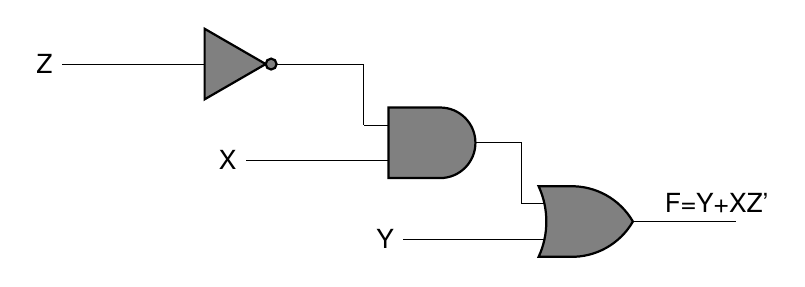
\begin{tikzpicture}
\ctikzset{
    logic ports=ieee,
    logic ports/scale=0.8,
    logic ports/fill=gray
}
 
% Logic ports
\node[not port] (nota) at (0,0){};
\node[and port] (anda) at (2.5,-1){};
\node[or port]  (ora) at (4.5,-2){};
 
\draw (nota.out) -| (anda.in 1);
\draw (anda.out) -| (ora.in 1);
 
\draw (ora.out) -- ++(1,0) node[near end,above]{F=Y+XZ'};
 
\draw (nota.in 1) -- ++(-1.5,0)node[left]{Z};
\draw (anda.in 2) -- ++(-1.5,0)node[left]{X};
\draw (ora.in 2) -- ++(-1.5,0)node[left] {Y};
 

\end{tikzpicture}
\begin{center}
Fig. 1 
\end{center}

\section{K-map Implementation}
Using the boolean logic output F can be expressed in terms of the inputs X,Y,Z with the help of the following Kmap.
\\
\\
\\
	 \begin{center}
     \begin{karnaugh-map}[4][2][1][$YZ$][$X$]
        \maxterms{0,1,5}
        \minterms{2,3,4}
        %\minterms{7,6}
        \terms{6}{$X$}
		\terms{7}{$X$}   
        \implicantedge{4}{4}{6}{6}
        \implicant{3}{6}
       
    \end{karnaugh-map}
\end{center}
%\end(document)
\begin{center}
Fig. 2
\end{center}



 \paragraph {Reducing the boolean Function}
    F=X'Y+XY'Z'\\
    F=X'Y(Z+Z')+XY'Z'\\
    X'YZ+X'YZ'+XY'Z'\\
 Reduced expression using K-maps is\\
 F=Y+XZ'\\

    
\section{Implementation}
  \begin{tabularx}{0.46\textwidth} { 
  | >{\centering\arraybackslash}X 
  | >{\centering\arraybackslash}X 
  | >{\centering\arraybackslash}X  | }


\hline
\textbf{Arduino PIN} & \textbf{INPUT} & \textbf{OUTPUT} \\ 
\hline
\textbf 2 & X & \\
\hline
\textbf 3 & Y & \\
\hline
\textbf 4 & Z & \\
\hline
\textbf 8 & & F \\
\hline
\end{tabularx}

\begin{center}
    Connections
\end{center}

    \paragraph{Problem-1}
    
    1. Connect the circuit as per the above table.\\
    2. Connect the output pin to LED\\
    3. Connect inputs to Vcc for logic 1, ground for logic 0\\
    4. Execute the circuit using the below code.\\
   
\begin{tabularx}{0.46\textwidth} { 
  | >{\centering\arraybackslash}X |}
  \hline
  https://github.com/aruniot099/FWC-1/blob/main/IDE/code\\
  \hline
\end{tabularx}

   \paragraph{Problem-2}
1. Change the values of X,Y,Z in the code and verify the Truth Table\\


\bibliographystyle{ieeetr}
\end{document}